\documentclass[journal]{IEEEtran}

% ---- Safe, minimal packages (ASCII only) ----
\usepackage[T1]{fontenc}
\usepackage[utf8]{inputenc}
\usepackage{lmodern}
\usepackage{graphicx}
\usepackage{amsmath,amssymb}
\usepackage{booktabs}
\usepackage{siunitx}
\usepackage[hidelinks]{hyperref}
\usepackage{cite}

\graphicspath{{./}{figs/}}

\title{A Comparative Review of DRAM and FeRAM: The Boundary between Volatile and Non-Volatile Memory and Future Perspectives}

\author{Shinichi~Samizo%
\thanks{S. Samizo is with Project Design Hub (Samizo–AITL), Japan. E-mail: \texttt{samizo-aitl@example.org}.}
}

\markboth{Draft for IEEE-style submission}{Samizo: DRAM vs FeRAM Comparative Review}

\begin{document}
\maketitle

\begin{abstract}
Dynamic Random-Access Memory (DRAM) is the workhorse of volatile memory, while ferroelectric memories (FeRAM and FeFET) offer CMOS-compatible non-volatility. This paper reviews DRAM and FeRAM from technology scaling and reliability to system-level use. We summarize key metrics (speed, retention, endurance, and energy/bit) and discuss hybrid hierarchies that combine DRAM performance with FeRAM persistence.
\end{abstract}

\begin{IEEEkeywords}
DRAM, FeRAM, FeFET, HfO2, retention, endurance, scaling, memory hierarchy.
\end{IEEEkeywords}

\section{Introduction}
% sections/intro.tex

\section{Introduction}

Memory hierarchies are central to computing systems. 
DRAM remains the dominant volatile memory due to speed, density, and scalability \cite{choi2022,kim2021_dram}. 
However, DRAM scaling faces limits as capacitors shrink; 3D DRAM concepts are explored to extend scaling \cite{iedm2023_dram}.

In parallel, doped HfO$_2$ ferroelectrics enabled FeRAM and FeFET with CMOS-friendly integration \cite{boscke2011,mueller2012}. 
These offer non-volatility with fast switching but face polarization variability, endurance, and TDDB concerns. 

This review contrasts DRAM and FeRAM at device and system levels and outlines hybrid use-cases. 
As an overview, Figs.~\ref{fig:speed_retention} and \ref{fig:energy_speed} conceptually illustrate the trade-offs in access speed, retention, and write energy, which will be detailed in Sec.~\ref{sec:comparison}.


\section{DRAM Technology and Scaling}
\section{DRAM Technology and Scaling}

DRAM technology has continually advanced through capacitor scaling, high-$k$ dielectrics, and process innovations. 
Maintaining sufficient cell capacitance while suppressing leakage becomes increasingly difficult at deep sub-20\,nm nodes \cite{choi2022}. 
To extend scaling, 3D DRAM concepts---stacking capacitor arrays analogous to 3D NAND---are explored \cite{iedm2023_dram}, 
though integration complexity and refresh overhead remain open challenges \cite{kim2021_dram}.

% ==== Fig.1: Speed (access time) vs. retention (TikZ/PGFPlots) ====
\begin{figure}[!t]
\centering
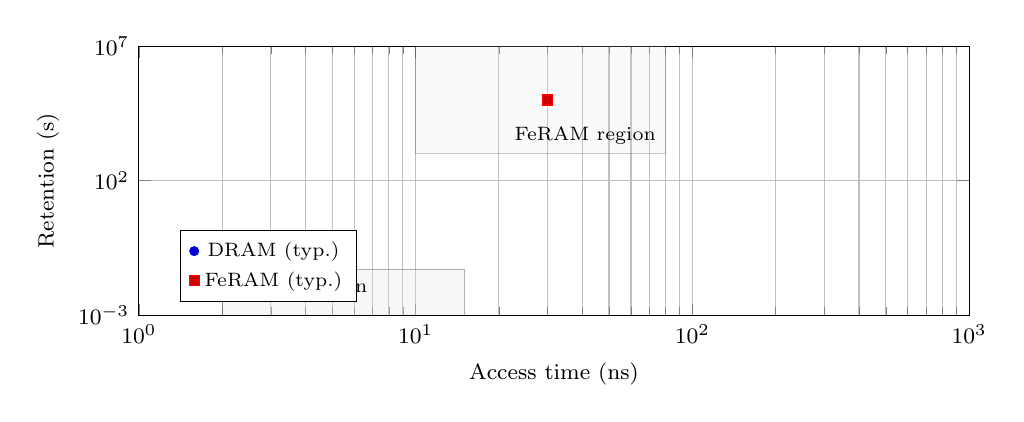
\begin{tikzpicture}
\begin{loglogaxis}[
  width=\linewidth,
  height=5.0cm,
  xlabel={Access time (ns)},
  ylabel={Retention (s)},
  xmin=1e0, xmax=1e3,
  ymin=1e-3, ymax=1e7,
  grid=both,
  legend style={at={(0.05,0.05)},anchor=south west, font=\scriptsize},
  label style={font=\footnotesize},
  tick label style={font=\footnotesize}
]
% Typical points (conceptual)
\addplot+[only marks,mark=*,mark size=1.6pt] coordinates {(5, 1e-2)};     
\addlegendentry{DRAM (typ.)}
\addplot+[only marks,mark=square*,mark size=1.8pt] coordinates {(30, 1e5)}; 
\addlegendentry{FeRAM (typ.)}

% DRAM region (conceptual)
\addplot [draw=black, fill=black!10, opacity=0.3] 
  coordinates {(2,1e-3) (15,1e-3) (15,5e-2) (2,5e-2)} -- cycle;
% FeRAM region (conceptual)
\addplot [draw=black, fill=black!10, opacity=0.2] 
  coordinates {(10,1e3) (80,1e3) (80,1e7) (10,1e7)} -- cycle;

\node[anchor=north west, font=\scriptsize] at (axis cs:2,5e-2) {DRAM region};
\node[anchor=south east, font=\scriptsize] at (axis cs:80,1e3) {FeRAM region};
\end{loglogaxis}
\end{tikzpicture}
\caption{Speed vs.\ retention (conceptual). DRAM is faster but requires refresh; FeRAM offers long retention at modest access times.}
\label{fig:speed_retention}
\end{figure}


\section{FeRAM Technology and Advances}
The discovery of robust ferroelectricity in doped HfO2 films enabled FeRAM and FeFET \cite{boscke2011,mueller2012}. FeFET cells provide 1T bit storage with non-volatility and fast reads; FeRAM capacitors offer low-voltage writes. Challenges include polarization variability, endurance in the 10^{12}–10^{13} range, and TDDB under high fields; recent work addresses device physics and integration routes toward memory and compute-in-memory.

\begin{figure}[!t]
  \centering
  \fbox{\rule{0pt}{1.10in}\rule{0.95\linewidth}{0pt}}
  \caption{Write energy per bit vs. write speed (placeholder). FeRAM/FeFET often sit at higher write energy than DRAM but provide non-volatility.}
  \label{fig:energy_speed}
\end{figure}


\section{Comparative Analysis: DRAM vs FeRAM}
\label{sec:comparison}
\section{Comparative Analysis: DRAM vs FeRAM}
\label{sec:comparison}

Table~\ref{tab:comparison} summarizes representative literature values for DRAM and FeRAM. Figures~\ref{fig:speed_retention} and \ref{fig:energy_speed} illustrate key trade-offs.

\begin{figure}[!t]
  \centering
  \includegraphics[width=\linewidth]{figs/fig_speed_retention}
  \caption{Speed vs.\ retention trade-off (representative, schematic).}
  \label{fig:speed_retention}
\end{figure}

\begin{figure}[!t]
  \centering
  \includegraphics[width=\linewidth]{figs/fig_energy_speed}
  \caption{Write energy per bit vs.\ write speed (representative, schematic).}
  \label{fig:energy_speed}
\end{figure}


\section{Hybrid Perspectives and Future Memory Hierarchies}
% sections/hybrid.tex
\section{Hybrid Perspectives and Future Memory Hierarchies}

Hybrid memory hierarchies aim to combine DRAM performance with FeRAM persistence. By placing FeRAM near the controller or adjacent to DRAM, systems can reduce refresh energy, enable instant-on features, and accelerate checkpointing and recovery for critical state.

% --- Fig.5: Hybrid hierarchy schematic (TikZ actual figure) ---
\begin{figure}[!t]
  \centering
  \begin{tikzpicture}[
    font=\footnotesize,
    box/.style={rounded corners, draw, minimum width=38mm, minimum height=9mm, align=center},
    >={Latex},
    node distance=6mm
  ]
    % Blocks
    \node[box, fill=gray!18] (cpu)  {CPU Registers / Cache};
    \node[box, fill=blue!12,  below=of cpu]  (dram) {DRAM\\(high-speed working set)};
    \node[box, fill=green!12, below=of dram] (feram){FeRAM / FeFET\\(near-memory, persistent)};
    \node[box, fill=yellow!18,below=of feram] (ssd)  {SSD / HDD\\(block storage)};

    % Vertical data path
    \draw[->] (cpu)  -- (dram);
    \draw[->] (dram) -- (feram);
    \draw[->] (feram) -- (ssd);

    % Side/bypass flows
    \draw[dashed,->] (cpu.east)  .. controls +(1,0.3)  and +(1,0.3)  .. (feram.east);
    \draw[dashed,->] (dram.east) .. controls +(1,0.3)  and +(1,-0.3) .. (ssd.east);

    % Notes
    \node[align=left, anchor=west] at ($(dram.east)+(1.2,0)$)
      {Refresh reduction\\Hot/Cold tiering};
    \node[align=left, anchor=west] at ($(feram.east)+(1.2,0)$)
      {Instant-on \& checkpoints\\Wear/retention mgmt.};
  \end{tikzpicture}
  \caption{Hybrid memory hierarchy where FeRAM near DRAM provides persistence and reduces refresh pressure.}
  \label{fig:hybrid_hierarchy}
\end{figure}

\subsection*{Benefits}
\begin{itemize}
  \item Reduced refresh overhead: cold pages and metadata can reside in FeRAM, cutting DRAM refresh traffic and standby power.
  \item Fast persistence: OS and application state can be checkpointed to FeRAM with microsecond-scale latency.
  \item Data resilience: FeRAM provides crash consistency for critical metadata and write-back buffers.
\end{itemize}

\subsection*{Constraints and trade-offs}
\begin{itemize}
  \item Endurance and variability: FeRAM endurance ($10^{12}$--$10^{13}$ cycles) is high but below effective DRAM activity levels.
  \item Write energy and latency: typically higher than DRAM; placement should bias read-mostly or cold data to FeRAM.
  \item Integration cost: ferroelectric layer/FeFET adoption adds process and reliability risks (e.g., high-field stress).
\end{itemize}

\subsection*{System directions}
\begin{itemize}
  \item Tiering policies using intensity/retention-aware placement and migration.
  \item Refresh co-optimization: shrink DRAM refresh for regions shadowed or backed by FeRAM.
  \item Controller/OS support for wear tracking, retention-aware placement, and error telemetry.
\end{itemize}


\section{Conclusion and Outlook}
% sections/conclusion.tex

DRAM will continue to dominate volatile working memory due to speed, density, and ecosystem maturity. HfO2-based FeRAM/FeFET offers a CMOS-compatible non-volatile complement with fast access, though variability, endurance dispersion, and integration limits remain active topics \cite{noheda2023,martin2020}. Hybrid hierarchies that pair DRAM for hot data with FeRAM for persistence can reduce refresh energy while enabling fast recovery paths.

Looking ahead, co-design across devices, controllers, and operating systems will be central: retention-aware placement, telemetry-driven reliability management, and low-latency persistence paths are promising directions to broaden deployment from embedded and edge to selected data-centric systems.


% --- References ---
\bibliographystyle{IEEEtran}
\bibliography{references}
\end{document}
